\documentclass[main]{subfiles}



\title[AutoML: Introduction]{AutoML Motivation}
\subtitle{Why AutoML?}
\author[Marius Lindauer]{Marius Lindauer}
\date{}

\titlebackground*{images/AutoML_AutoDL}

%\institute{}
%\date{}

\begin{document}
	
	\maketitle
	

%----------------------------------------------------------------------
%----------------------------------------------------------------------
\begin{frame}[c]{A Definition of \alert{Automated} Machine Learning}

\begin{center}
AutoML contributes to the efficient, reproducible, and systematic design of effective intelligent systems by creating a general automated development process, targeting the full machine learning workflow. 
\end{center}

\end{frame}
%-----------------------------------------------------------------------

%----------------------------------------------------------------------
\begin{frame}[c]{Advantages of AutoML}


In the development of new ML applications, AutoML improves...

\begin{itemize}
    \item[\emoji{rocket}] \textbf{Efficiency \& Effectiveness} -- AutoML has been shown to outperform humans in machine learning and data science competitions!
    \item[\emoji{abacus}] \textbf{Consistent Systematics} -- Less (human) bias or unsystematic evaluation
    \item[\emoji{open-book}] \textbf{Reproducibility} -- Software can run again under the same settings, humans cannot  
\end{itemize}

\medskip
\pause 

$\leadsto$ This has led to a broader use of ML methods:
\begin{itemize}
    \item Faster development cycles
    \item Less required ML expertise
    \item Not only limited to computer scientists
\end{itemize}

\end{frame}
%-----------------------------------------------------------------------
%----------------------------------------------------------------------
\begin{frame}[c]{\emoji{rocket}Efficiency -- Success of AutoML Systems}

\begin{columns}
\column{0.6\textwidth}

\begin{itemize}
    \item In 2024, AutoGluon \liturl{Erickson et al}{https://auto.gluon.ai/stable/index.html} won a Top 3 position in 17 out of 21 tabular \liturl{Kaggle}{https://www.kaggle.com/} competitions 
    \begin{itemize}
        \item Each competition had an average of 1\,500 human teams
    \end{itemize}
    \item AutoGluon, as one of the most successful AutoML packages in 2024, was used by major companies such as NVIDIA, Intel, Capcom, Mitsubishi, Oracle, Pinterest and others
\end{itemize}

\column{0.4\textwidth}

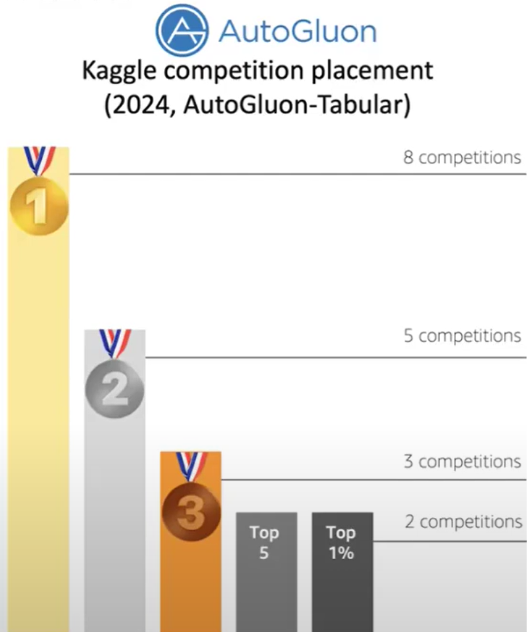
\includegraphics[width=1.0\textwidth]{images/autogluon_results.png}

\end{columns}

\end{frame}
%-----------------------------------------------------------------------
%----------------------------------------------------------------------
\begin{frame}[c]{\emoji{abacus}Systematic}

\begin{columns}

\column{0.4\textwidth}

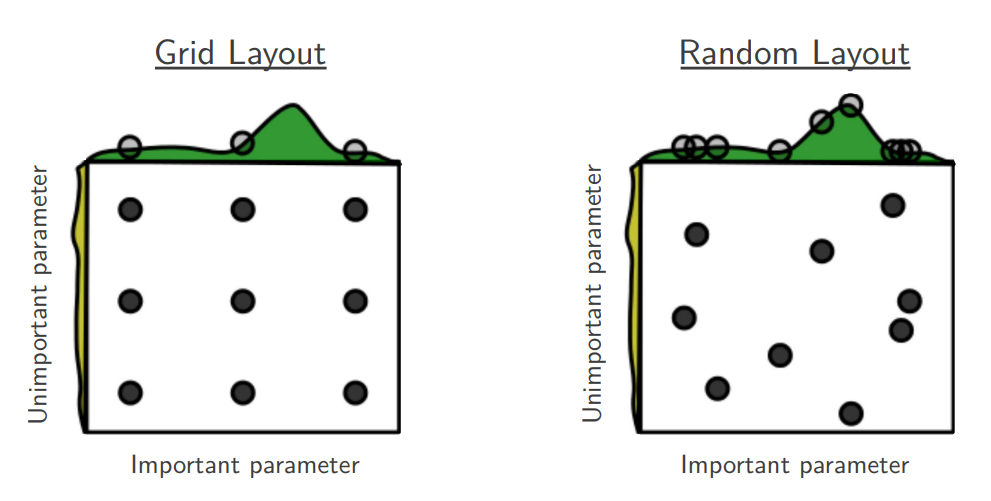
\includegraphics[width=1.0\textwidth]{images/grid_vs_random_bergstra12.png}

\liturl{Bergstra and Bengio et al. 2012}{https://www.jmlr.org/papers/volume13/bergstra12a/bergstra12a.pdf}

\column{0.6\textwidth}

\begin{itemize}
    \item Behind each AutoML approach, there is a systematic assumption on how to proceed
    \begin{itemize}
        \item Grid search: structured pre-defined grid for uniform exploration
        \item Random search: unstructured, uniform exploration
        \item Bayesian Optimization: Trade-off between exploration and exploitation
        \item ...
    \end{itemize}
    \item This is in contrast to unreproducible human bias, which could lead to suboptimal decisions (e.g.,\\ ``I have learned about Transformers, so I'm trying only Transformers'')
\end{itemize}
    
\end{columns}

\end{frame}
%-----------------------------------------------------------------------
%----------------------------------------------------------------------
\begin{frame}[c]{\emoji{open-book} Reproducibility}

\begin{columns}

\column{0.5\textwidth}

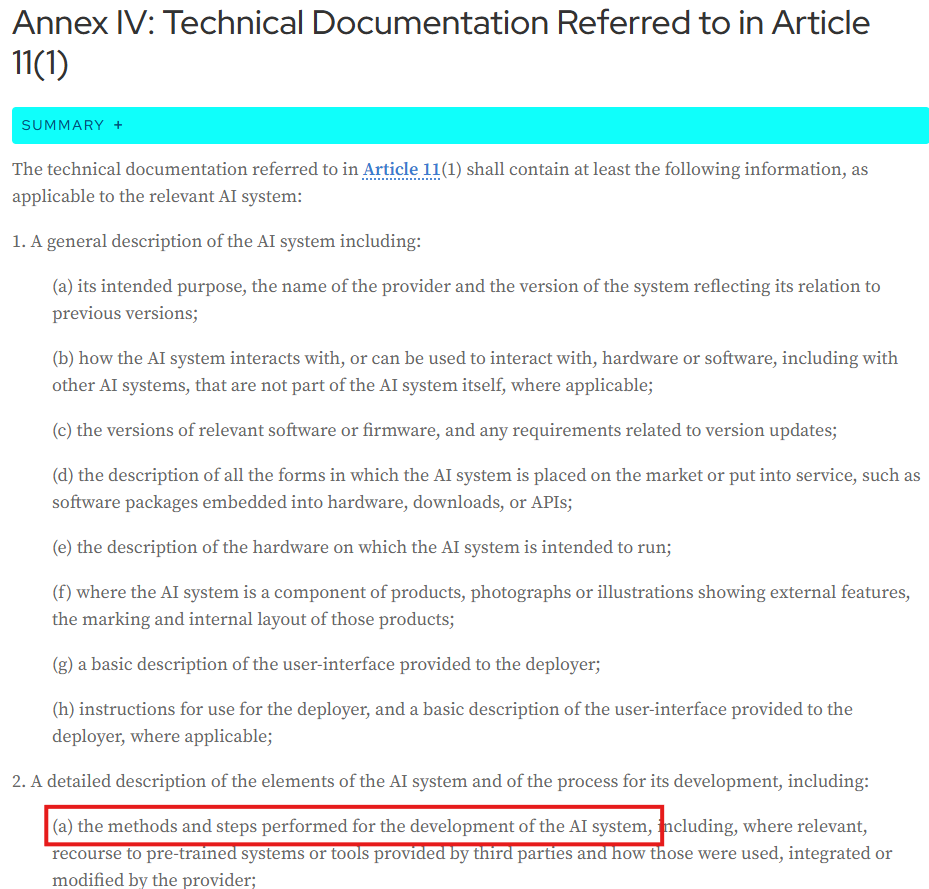
\includegraphics[width=0.8\textwidth]{images/eu_ai_act.png}

\liturl{EU}{https://artificialintelligenceact.eu/annex/4/}

\column{0.5\textwidth}

\begin{itemize}
    \item Reproducibility of ML development is becoming more and more important!
    \item Systems are more reproducible than any human!
    \item EU AI Act requires documentation -- AutoML can help with that!
    \item Research conference and journal also highly value reproducibility!
\end{itemize}
    
\end{columns}

\end{frame}
%-----------------------------------------------------------------------

%----------------------------------------------------------------------
\begin{frame}[c]{Use of (Auto)ML}

\begin{columns}

\column{0.6\textwidth}


\includegraphics[width=1.\textwidth]{images/hpo_cites.png}


\column{0.4\textwidth}

\begin{itemize}
    \item For example, hyperparameter optimization, as a subfield of AutoML, is commonly used in many disciplines using ML by now
    \begin{itemize}
        \item See for example citations of the HPO survey \liturl{Bischl et al. 2023}{https://wires.onlinelibrary.wiley.com/doi/full/10.1002/widm.1484}
    \end{itemize}
    \item (Parts of) AutoML are well established and enable ML projects that would not have been feasible a decade ago
    \end{itemize}
    
\end{columns}

\end{frame}
%-----------------------------------------------------------------------

%----------------------------------------------------------------------
\begin{frame}{Summary} 

Most important insights from this video:

\begin{enumerate}
    \item AutoML is a key ingredient for developing new ML applications
    \item It improves efficiency and effectiveness, but also helps in satisfying legal obligations or expectations from the academic community
    \item AutoML is important for both ML developers and domain experts from other fields
\end{enumerate}


\end{frame}

\end{document}
